%%%%%%%%%%%%%%%%%%%%%%%%%%%%%%%%%%%%%%%%%%%%%%%%%%%%%%%%%%%%%%%%%%%%%%%%%%%%%%
%arxiv
\documentclass[a4paper,11pt]{article}
% \pdfoutput=1
\usepackage{jcappub}

%%%%%%%%%%%%%%%%%%%%%%%%%%%%%%%%%%%%%%%%%%%%%%%%%%%%%%%%%%%%%%%%%%%%%%%%%%%%%%

\newcommand{\apjs}{ApJ Supplement}
\newcommand{\apj}{ApJ}
\newcommand{\aap}{AAP}
\newcommand{\mnras}{MNRAS}
\newcommand{\prd}{PRD}
\newcommand{\gadget}{{\small GADGET}}
\newcommand{\mpgadget}{{\small MP-GADGET}}

\newcommand{\km}{k_{max}}

\newcommand{\vect}[1]
  {\mbox{\boldmath ${#1}$}}
\newcommand{\matr}[1]
  {\mbox{\bf \sf{#1}}}
\newcommand{\eq}[1]
  {Eq.~(\ref{equation:#1})}
\newcommand{\eqs}[1]
  {Eqs~(\ref{equation:#1})}
\newcommand{\sect}[1]
  {section~\ref{section:#1}}
\newcommand{\sects}[1]
  {sections~\ref{section:#1}}
\newcommand{\tabl}[1]
  {{\mbox Table~\ref{table:#1}}}
\newcommand{\tabls}[1]
  {{\mbox Tables~\ref{table:#1}}}
\newcommand{\fig}[1]
  {Fig.~\ref{Figure:#1}}
\newcommand{\figs}[1]
  {Figs.~\ref{Figure:#1}}
\newcommand{\sourcesection}[1]{\noindent {\em{#1}} ---}

\def\jcap{JCAP}        % Journal of Cosmology and Astro-Particle Physics

\newcommand{\Lya}{Lyman-$\alpha$}
\newcommand{\Msun}{\, h^{-1} M_\odot}
\newcommand{\Zsun}{Z_\odot}
\newcommand{\NHunit}{cm$^{-2}$}
\newcommand{\sLLS}{\sigma_\mathrm{LLS}}
\newcommand{\Mpc}{\,\mathrm{Mpc}}
\newcommand{\Mpch}{\, h^{-1} \mathrm{Mpc}}
\newcommand{\kpch}{\, h^{-1}\mathrm{kpc}}
\newcommand{\hMpc}{\, h \mathrm{Mpc}^{-1}}
\newcommand{\kms}{km~s$^{-1}$}
\newcommand{\NHI}{N_\mathrm{HI}}

\newcommand{\spb}[1]{\textcolor{red}{[\bf SPB: #1]} }
\newcommand{\AFR}[1]{\textcolor{blue}{[\bf AFR: #1]} }
\newcommand{\YF}[1]{\textcolor{green}{[\bf YF: #1]} }

\newcommand{\edit}[1]{#1}

%opening
\title{Lagrangian Glasses for N-body Simulations of Baryons and Dark Matter}

\author[a,1]{Simeon Bird,\note{Corresponding author}}
\author[b]{Yu Feng}
\author[c]{Chris Pederson}
\author[c]{Andreu Font-Ribera}
\affiliation[a]{Department of Physics \& Astronomy, University of California Riverside,\\ Riverside, CA 92521, USA}
\affiliation[b]{Berkeley Center for Cosmological Physics, University of California Berkeley, \\Berkeley, CA 94720, USA}
\affiliation[c]{Department of Physics \& Astronomy, University College London,\\Gower Street, London WC1E 6BT, UK}

\emailAdd{sbird@ucr.edu}
\emailAdd{yfeng1@berkeley.edu}
\emailAdd{christian.pedersen.17@ucl.ac.uk}
\emailAdd{a.font@ucl.ac.uk}

\abstract{
XXXX
}

\begin{document}

\maketitle

\section{Introduction}

Cosmological N-body simulations are a well-established technique for understanding non-linear structure formation. A common technique for N-body simulations is model a single fluid, corresponding to a combination of cold dark matter (CDM) and baryons, under gravity, under the approximation that these two components trace each other. Hydrodynamic simulations follow baryons using a separate particle species, but frequently use the same initial transfer function for each species \cite[e.g.][]{Emberson:2018}.

However, at early times the baryons couple to radiation, while the CDM does not. This both induces the baryon acoustic oscillation (BAO) peak  and reduces the clustering of baryonic matter on scales less than the comoving horizon scale at recombination.
As the Universe evolves, the process of structure formation gradually erases the difference between baryons and CDM, as each species traces ever more accurately the total gravitational potential. By $z=0$ the power spectrum of baryons and CDM differs by less than $1\%$. Nevertheless, at higher redshift they differ substantially, by up to $8\%$ at $z=10$ and $3\%$ at $z=2$ for $ k > 0.02$ k/Mpc.

As observational probes of the Universe reach ever higher redshift, these differences may become more relevant. However, naively modelling separate transfer functions for each species does not reproduce a key prediction of linear theory, the evolution of the offset in power between the CDM and baryon species \cite{OLeary:2012, Angulo:2013}.  The practical impact of this effect is fortunately reduced because the coupling conserves total momentum, and thus shows the correct evolution of the total matter spectrum. However, some cosmological probes, such as the \Lya~forest \cite{PD2013}, or $21$-cm power spectrum are sensitive specifically to neutral gas, whose power spectrum differs from the total matter power by up to $10\%$. Here we investigate the effect on the \Lya~forest, and leave the $21$-cm power spectrum for future work.

Refs~\cite{OLeary:2012, Angulo:2013} showed that linear theory can be reproduced by increasing the gravitational softening length of the particles at high redshift. This is done adaptively, setting the baryonic softening length equal to the SPH smoothing length of the baryonic particles. This effectively disables the short range gravitational force at high redshift, when the Universe is homogeneous and thus SPH smoothing lengths are of order the mean inter-particle spacing. We emphasize that on cosmological scales this procedure cannot be justified on the basis of hydrodynamics. The coupling effect is purely gravitational, and persists even if, as in the simulations of Ref.~\cite{Angulo:2013} and the ones presented here, hydrodynamical pressure forces are disabled. Adaptive softening is thus simply an easy way of increasing the softening only at the high redshifts where the problem is most acute. Since the small-scale gravitational force is disabled at high redshift, adaptive softening strongly suppresses the small-scale clustering of the baryons in low density regions outside galaxies. This may make it unsuitable for some applications, in particular simulations of the \Lya~forest. Nevertheless, adaptive softening is widely used in recent simulations \cite[e.g][]{Paco:2018}.\footnote{Ref.~\cite{Valkenburg:2017} instead achieved the same effect by setting the cutoff distance for the small-scale force to a small fraction of the PM grid size.}

An alternative resolution to this problem was proposed by Ref.~\cite{Yoshida:2003}. They showed that the desired relative power between baryons and cold dark matter could be achieved by initializing the particles using two independent Lagrangian glasses, rather than the more standard offset grids. The effect of particle couplings propagates to large scales due to the regular grid structure of the simulation, which means that each low-mass (baryonic) particle is equally perturbed by the local effect of the nearest high mass (cold dark matter) particles. A local perturbation is thus replicated across the box and shows up as a large scale offset from the desired growth. Many of our results are implicit in Ref.~\cite{Yoshida:2003}. However, they did not consider large scales and thus did not include the effect of species and scale dependent velocity transfer functions as we do here.
We show that initializing the baryons using a Lagrangian glass rather than a grid offset from the CDM allows a simulation to reproduce the ratio between CDM and baryons predicted by linear theory. The noise inherent in a glass distribution is reduced by using a glass only for the baryons, not for the CDM. To further prevent chance juxtapositions of CDM and baryon particles we perform reverse-gravity timesteps on the combined particle distributions.

We consider other methods for resolving the particle discrepancy, showing that it is not due to force inaccuracy. We investigate an alternative technique to reproducing the linear theory prediction of the baryon-CDM offset is to over-sample the CDM relative to baryons by a factor of $\Omega_\mathrm{CDM}/\Omega_\mathrm{b}$, so that each particle species has equal mass.

% This means that each particle species has roughly the same mass and thus the inaccuracies resulting from differing mass particles are removed.

Other possibilities for the initial particle distribution have also been proposed. Ref.~\cite{Hansen:2007} used a quaquaversal tiling of three dimensional space, which we do not consider as it restricts the total number of particles to a power of two. Ref.~\cite{Liao:2018} used a capacity constrained Voronoi tessellation, which preserves most of the good properties of a Lagrangian glass. We do not use it here only because it is not obvious how to generalize it to two fluids. Finally, Ref.~\cite{Zennaro:2017} avoid the problem by ``backscaling'', where each species is scaled separately by the requisite factor so that the simulation output at $z=0$ exactly matches the linear theory prediction.

The rest of this paper proceeds as follows: in Section~\ref{sec:methods} we discuss in detail our techniques for initialising cosmological simulations. In Section~\ref{sec:glass} we review the formation of a glass file. Section~\ref{sec:particles} explains how we set the initial displacements and velocities of the particles. Section~\ref{sec:simulations} describes our example simulation suite. Our results are described in Section~\ref{sec:results}. Section~\ref{sec:matterpower} shows how each of the considered initialisation techniques affects the matter power spectrum. Section~\ref{sec:lymanalpha} shows the effect on the \Lya~forest of a species-dependent transfer function. We conclude in Section~\ref{sec:conclude}.

% Simulations generally wish to achieve equal average spatial separation and thus equal fractional mass resolution in baryons and CDM. As $\Omega_\mathrm{b} < \Omega_\mathrm{CDM}$, this implies that the mass of baryonic particles differs from the mass of CDM particles.
%  These unequal masses can induce unphysical coupling of the lower mass (baryonic) particles to the higher mass (CDM) particles \cite{OLeary:2012}, in extreme cases binding the lighter particles to orbiting the heavier ones. A simple analytic derivation of this effect is shown in Appendix B of Ref.~\cite{OLeary:2012}.
%
% A minority interested in high redshift structure growth initialize CDM and baryons using the transfer functions for their respective species. In this case accurate evolution requires also using separate velocity transfer functions for the CDM and baryons. In an attempt to regularise tree construction and avoid unphysical two-body couplings, baryonic and CDM particles are initially offset by half the mean inter-particle spacing.
%
% Ref.~\cite{Angulo:2013} showed that the ratio between the baryon power spectrum, $P_b(k)$, and the CDM power spectrum $P_\mathrm{CDM}(k)$, in Gadget-3 \cite{Springel:2005} simulations does not by default agree with the predictions of linear theory, due to this spurious inter-particle coupling.

%I feel strongly that Angulo & Hahn simply wrote a wrong paper - our results agree much better with Yoshida 2003 than them.
%We have never been able to reproduce their results and when we use a glass file we get the right answer.
%They I think probably used the wrong velocity transfer functions.

\section{Methods}
\label{sec:methods}

In this Section we describe our methods for initializing cosmological simulations, as well as the simulations we run.
The basic algorithm of our preferred setup is similar to that presented in Ref~\cite{Yoshida:2003} and is as follows:
\begin{enumerate}
 \item Produce a (homogeneous) distribution of CDM particles arranged in a regular grid.
 \item Produce a (homogeneous) distribution of gas particles from a Lagrangian glass.
 \item Evolve the mixed distribution of both types of particles using a reversed gravitational force, as when generating a Lagrangian glass. This avoids random close juxtapositions of CDM and baryon particles.
 \item Set the velocity of the baryon and CDM particles using the scale-dependent velocity transfer function specific to each species.
  \item Displace the baryon and CDM particles using the displacement transfer function specific to each species.
\end{enumerate}

Section~\ref{sec:glass} describes Steps 1-3, the initialization of our undisplaced particle tables from grid and glass files. Steps 4-5, the generation of the velocity and position displacements, are described in Section~\ref{sec:particles}.

\subsection{Grid and Glass Particle Distribution Generation}
\label{sec:glass}

We generate glass particle distributions following \cite{White:1994}. A gravitationally interacting N-particle system is evolved with the sign of gravity reversed, so that each particle feels a repulsive gravitational force from every other particle. We have implemented this gravitational force evolution directly into our initial conditions code and it thus uses the particle-mesh algorithm from our N-body code, MP-Gadget. The initial particle distribution before glass generation is a regular grid with the positions of each particle randomized over three mean inter-particle spacings. A symplectic leap-frog is run with a kick-drift-force-kick arrangement for fourteen timesteps. The velocity kick includes a damping term proportional to the velocity to avoid particle positions oscillating around the minimum. The velocity produced by the glass evolution is zeroed after the glass generation is complete. The reverse gravity evolution is done for $14$ timesteps, the smallest that produced a small-scale noise power spectrum in good agreement with the expected $k^4$ shape.

This procedure can be applied separately to both CDM and baryons, generating two uniform homogeneous gas distributions.
Although the distribution of each individual particle species is homogeneous, there is no guarantee that this property also applies to the total particle distribution. The original benefit of a glass, low residual force between all particles, does not hold for two combined glasses \cite{Yoshida:2003} as particles of one species may occasionally, by chance, be initialized extremely close to a particle of a different species. This causes two types of problems: the first is that close pairs of particles causes the computation of the gravitational force to be computationally expensive. The second is that artificial structure will be seeded at some level in the small regions around the close particles, causing a deviation from linear theory on small scales.

We investigated generating a single coherent glass file containing both species of particle. In this glass file both particle species are placed at random and then evolved with reversed gravity to a single, coherent, homogeneous distribution. However, this contained no mechanism for keeping the distribution of each species homogeneous, and thus produced a density map which had overdensities of baryons exactly compensated by overdensities of cold dark matter. This in turn led to a very noisy power spectrum estimation as not all modes were fully sampled. Furthermore, in a realistic hydrodynamical simulation it would have caused, for example, formation of dark matter halos containing no baryons.

Ref.~\cite{Yoshida:2003} proposed a resolution to reduce chance alignments of two particle species. After generating two separate homogeneous glass files, they ran a single reversed-gravity timestep on the combined particle distribution. This ensures that particles which are exceptionally close by chance are disrupted, but does not disrupt the overall glass distribution of the simulation. We perform $14$ reversed gravity timesteps on the combined particle distribution, so that the overall particle distribution is homogeneous.

Lacking the symmetry of a regular cubic grid, glass files produce spurious noise proportional to $k^4$ \cite{Peebles:1993}. Since our use of a glass distribution is solely designed to reproduce the linear theory offset between baryons and cold dark matter, we can reduce the glass noise by using a regular grid for the cold dark matter.\footnote{A grid also has an associated Fourier-space systematic: a broad peak at the grid scale. However, this is eventually erased by non-linear structure growth.} This is advantageous as at high redshift the cold dark matter dominates the linear theory power spectrum. Glass noise is still present, but at a reduced level because baryons are only $\sim 1/6$ of the total matter. We also show that in practice hydrodynamical forces further suppress the small scale power in baryons, effectively removing the $k^4$ noise power. In practice for realistic particle loads we found that the noise from the glass quickly became subdominant to the physical power spectrum from structure formation, but we use a regular grid for the CDM nevertheless.

% We also considered using $4$ timesteps rather than $14$ timesteps for the reversed gravity evolution of the combined CDM grid and baryonic glass. We found minimal difference in the final power spectra, but the extra timesteps did moderately reduce the number of close particle pairs in the simulation with some improvements in computational time, hence we chose to use $14$ timesteps for the combined particle distribution. \YF{this would show up as a deviation from k ** 4 power. I think we can add a figure showing the glass power vs k**4 with 4 and 14 steps. e.g. a polished version of cell 51 in the notebook. 3-3-2 is the configure we use.}

\subsection{Initialization of Particle Velocities and Displacements}
\label{sec:particles}

Key to reproducing linear theory is the correct initialization of particle velocities and displacements. Since there are several approximations current in the literature, and the velocity transfer functions in particular are not trivial, we here review the linear results.

We initialize both displacements and velocities directly using the transfer functions from the linear Boltzmann code CLASS \cite{CLASS}, corresponding to the solutions of the equations of linear cosmological perturbation theory in synchronous gauge. We apply a species-independent boost to the velocities, as the CLASS transfer functions are generated in a frame comoving with the cold dark matter. Following the notation of Ref.~\cite{Ma:1995}, we set:
\begin{align}
 v_\mathrm{CDM} = \dot{\delta}_\mathrm{CDM}  &= - \frac{\dot{h}}{2} \\
 v_\mathrm{b} = \dot{\delta}_\mathrm{b}  &= - \theta_\mathrm{b} - \frac{\dot{h}}{2}
\end{align}
where $\dot{h}$ and $\theta_\mathrm{b}$ are set using the relevant columns in the CLASS transfer functions.
Particle displacements are set using the columns for $\delta_\mathrm{CDM, b}$. Note that each of these quantities is fully scale-dependent, so that the scale-dependence of the velocity perturbations is automatically included without having to numerically differentiate the growth factor\footnote{See: \protect\url{https://github.com/MP-Gadget/MP-Gadget/blob/FirstDOI/libgenic/power.c\#L204}.}.

We do not use the common Zel'dovich approximation, which is to assume a scale-independent proportionality of the velocity transfer function to the displacement transfer functions
\begin{equation}
 v = a H(a) \frac{d \ln D_1(a)}{d \ln a} x
\end{equation}
where $x$ is the particle displacement and $D_1(a)$ is the growing mode total matter linear growth factor\footnote{Sometimes this is further approximated as $\Omega_M^{3/5}$, which is indefensible today.}. The growth function for individual species is not the total growth function, so this introduces an inaccuracy in the relative velocities of the baryons and CDM.

We do not use second-order Lagrangian perturbation theory \cite{Scoccimarro:1998}, despite its reduced transients as, to our knowledge, the full species specific velocity and displacement second order transfer functions, including baryon-CDM cross-terms, do not exist in the literature. We defer this to future work.

\subsection{Example Simulations}
\label{sec:simulations}

Our primary test simulations are performed with $2\times 256^3$ particles and box sizes of $300$ Mpc/h (comoving). Initial conditions are generated at $z=99$ and we compare to linear theory power spectra and transfer functions generated using CLASS \cite{CLASS}. We assume a periodic box and a standard $\Lambda$CDM cosmology with $\Omega_\mathrm{M} = 0.3$, $h = 0.67$, $n_s = 0.97$ and $\sigma_8 = 0.8$. We have set $\Omega_\mathrm{b} = 0.05$ so that $\Omega_{\mathrm{CDM}}/ \Omega_\mathrm{b} = 5$. For the majority of our tests accelerations are purely gravitational, despite including a baryonic particle component. Cooling, star formation and galaxy formation are disabled. To show the effect of pressure forces we perform a single simulation with hydrodynamics enabled. Hydrodynamics is included using Smoothed Particle Hydrodynamics with a cubic kernel, following \cite{Springel:2005}.

Our simulations are performed with the N-body code MP-Gadget and initial conditions were generated with MP-GenIC \cite{yu_feng_2018_1451799}. MP-Gadget is descended from P-Gadget3 \cite{Springel:2005}, with heavy modifications for scalability and force accuracy. In particular, as described in Ref.~\cite{Bird:2018}, the force tree is rebuilt completely every timestep, rather than nodes being moved according to the average particle velocity.

Our full set of simulations is shown in Table~\ref{tab:simulations}. To demonstrate that we reproduce the results of the literature, \texttt{TWOGRID} was a simulation with species-specific transfer functions and an undisplaced particle distribution of two offset grids. The \texttt{ADAPTIVE} simulation used the same initial conditions but evolved them using an adaptive gravitational softening set to match the SPH smoothing length.

We then performed simulations using the setup described in Section~\ref{sec:glass}, with pre-displacement CDM particles on a regular grid and pre-displacement baryon particles on a Lagrangian glass (\texttt{HALFGLASS}). To confirm that our results continue to hold on larger scales we performed a simulation (\texttt{BIGGLASS}) with a box of $1$ Gpc/h (a scale large enough that the baryon and CDM transfer functions are approximately equal on scales of the box) and $768^3$ particles. To confirm that the effect of pressure forces (\texttt{HYDROGLASS}) uses the same setup with hydrodynamics enabled for the baryonic particles.

The \texttt{UNDERSAMP} simulation used an alternative method for correctly reproducing the linear theory prediction for the ratio between CDM and baryons, undersampling the baryonic particles so that each individual CDM and baryon N-body particles have the same mass. For this simulation the pre-displacement CDM and baryon particles were initialized on offset grids, as for the \texttt{TWOGRID} simulation.

Finally, we performed two simulations adapted for the \Lya~forest, in a $120$ Mpc/h box with $2\times 512^3$ particles. These parameters were chosen so that the box was large enough to still include some portion of the BAO, while having sufficient resolution to roughly model the forest. One simulation (\texttt{FOREST}) used species specific transfer functions. A second (\texttt{TOTFOREST}) initialized both CDM and baryon particles with the total matter transfer function, following standard practice in the \Lya~field. Both simulations include radiative cooling following \cite{Katz:1996}, a self-shielding correction from \cite{Rahmati:2013} and a simplified star formation criterion which immediately turns all gas with an over-density $\Delta > 1000$ and a temperature $T < 10^5$ K into stars \cite{Viel:2004}. A uniform meta-galactic ultra-violet background was assumed following Ref.~\cite{Puchwein:2018}.

\begin{table}
\begin{center}
\begin{tabular}{|l|c|c|c|l|}
\hline
Name & Box & $N_\mathrm{CDM}^{1/3}$ & $N_\mathrm{baryon}^{1/3}$ & Comments  \\
\hline
\texttt{TWOGRID}    &   $300$ & $256$ & $256$ & Two offset particle grids. \\
\texttt{ADAPTIVE}    &   $300$ & $256$ & $256$ & As TWOGRID but adaptive gas softenings. \\
\texttt{HALFGLASS}  &   $300$ & $256$ & $256$ & Baryons on a glass, CDM on a grid, see text. \\
\texttt{BIGGLASS}  &   $1000$ & $768$ & $768$ & As HALFGLASS. \\
\texttt{HYDROGLASS}  &   $300$ & $256$ & $256$ & As HALFGLASS, but with pressure forces enabled. \\
\texttt{UNDERSAMP}  &   $300$ & $256$ & $150$ & Two offset particle grids, same particle masses. \\
\texttt{FOREST}  &   $120$ & $512$ & $512$ & As HALFGLASS but with \Lya~forest physics. \\
\texttt{TOTFOREST}  &   $120$ & $512$ & $512$ & Total matter transfer functions and \Lya~forest. \\
\hline
\end{tabular}
\end{center}
\caption{Table of simulations. Box size is in comoving Mpc/h. Details are explained in the text}
\label{tab:simulations}
\end{table}

\section{Results}
\label{sec:results}

\subsection{Matter Power Spectra}
\label{sec:matterpower}

\begin{figure}
  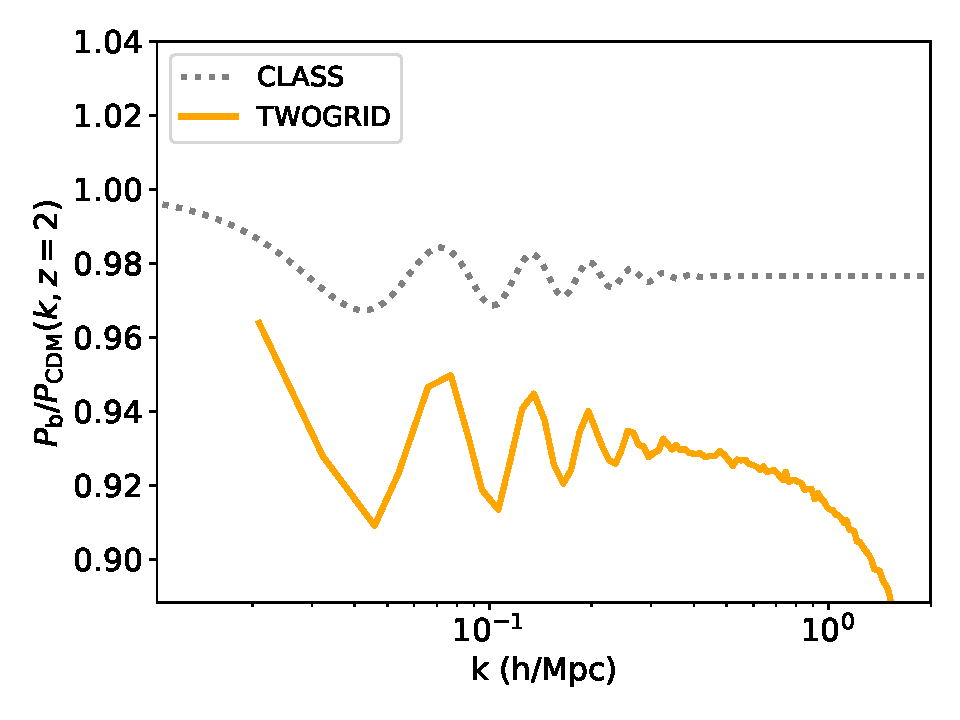
\includegraphics[width=0.5\textwidth]{plots/literature_2_relpower.pdf}
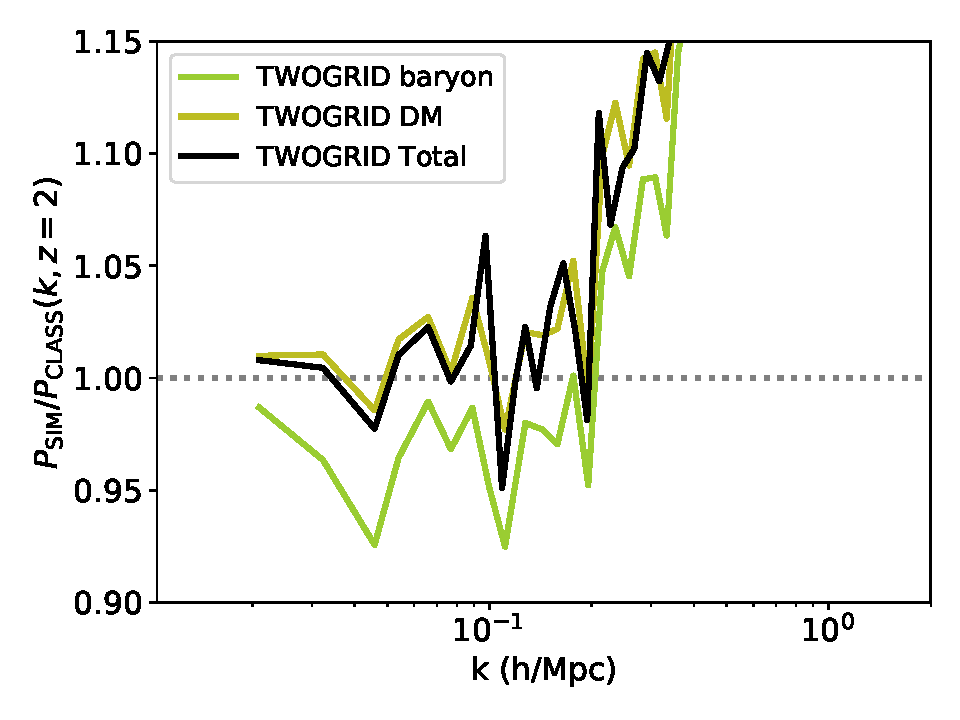
\includegraphics[width=0.5\textwidth]{plots/literature_2_class.pdf}
\caption{Results for the TWOGRID simulation, which initializes particles on two regular grids, offset by half a grid spacing. (Left) Ratio of baryon to CDM power spectra, $P_\mathrm{bar}/P_\mathrm{CDM}(k)$, at $z=2$ for the simulation (solid) and linear theory from CAMB (dash). (Right) Ratio of simulated to linear power spectra, $P_\mathrm{sim}/P_\mathrm{CLASS}(k)$ for gas (orange) and CDM (blue).}
  \label{fig:offsetgrids}
\end{figure}

\begin{figure}
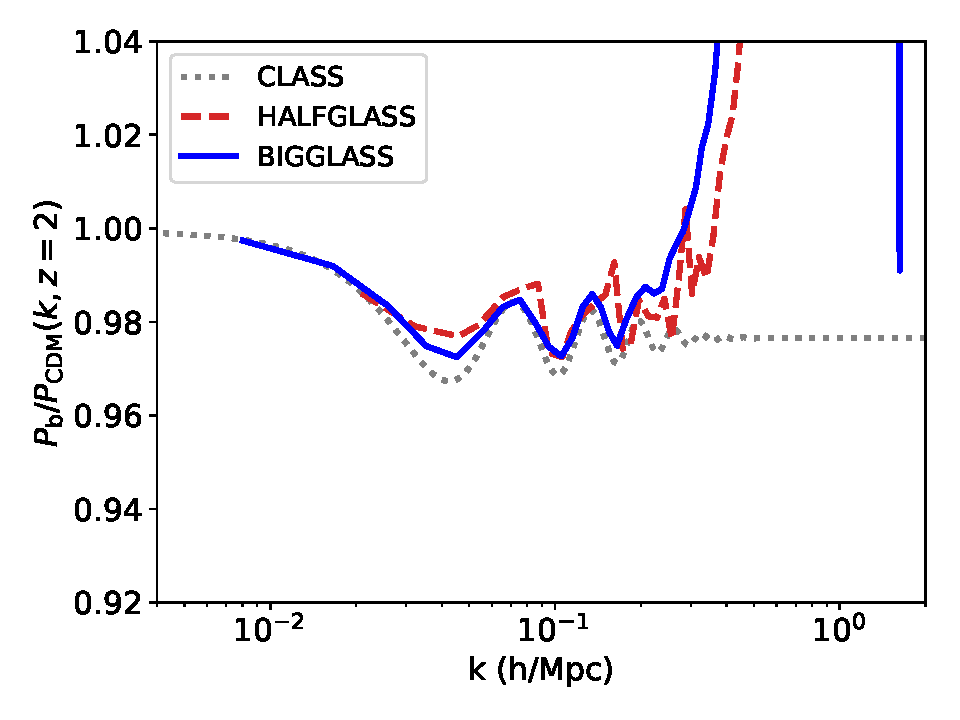
\includegraphics[width=0.5\textwidth]{plots/halfglass_2_relpower.pdf}
  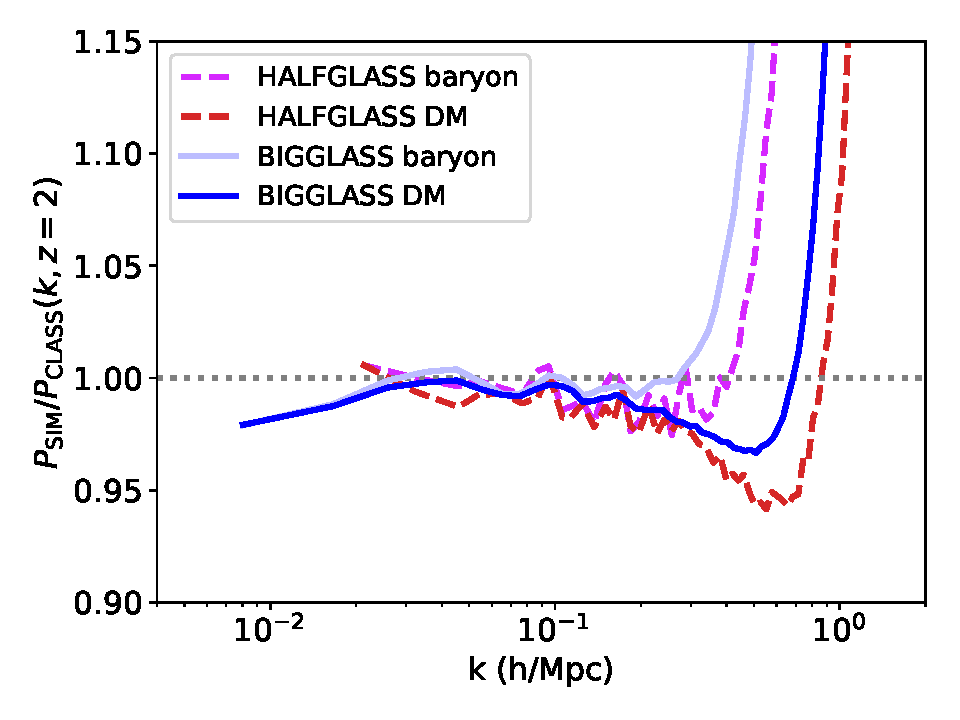
\includegraphics[width=0.5\textwidth]{plots/halfglass_2_class.pdf}
\caption{Results for our preferred simulation setup, where CDM is initialised with a regular grid and baryons are initialised with a glass. Shown are the HALFGLASS simulation, with $2\times 256^3$ particles in a $300$ Mpc/h box and the BIGGLASS simulation, with $2\times 768^3$ particles in a $1000$ Mpc/h box. (Left) Ratio of gas to CDM power spectra, $P_\mathrm{bar}/P_\mathrm{CDM}(k)$, at $z=2$ for the simulation (solid) and linear theory from CAMB (dash). (Right) Ratio of simulated to linear power spectra, $P_\mathrm{sim}/P_\mathrm{CLASS}(k)$ for gas (orange) and CDM (blue).}
  \label{fig:baryonglass}
\end{figure}

\begin{figure}
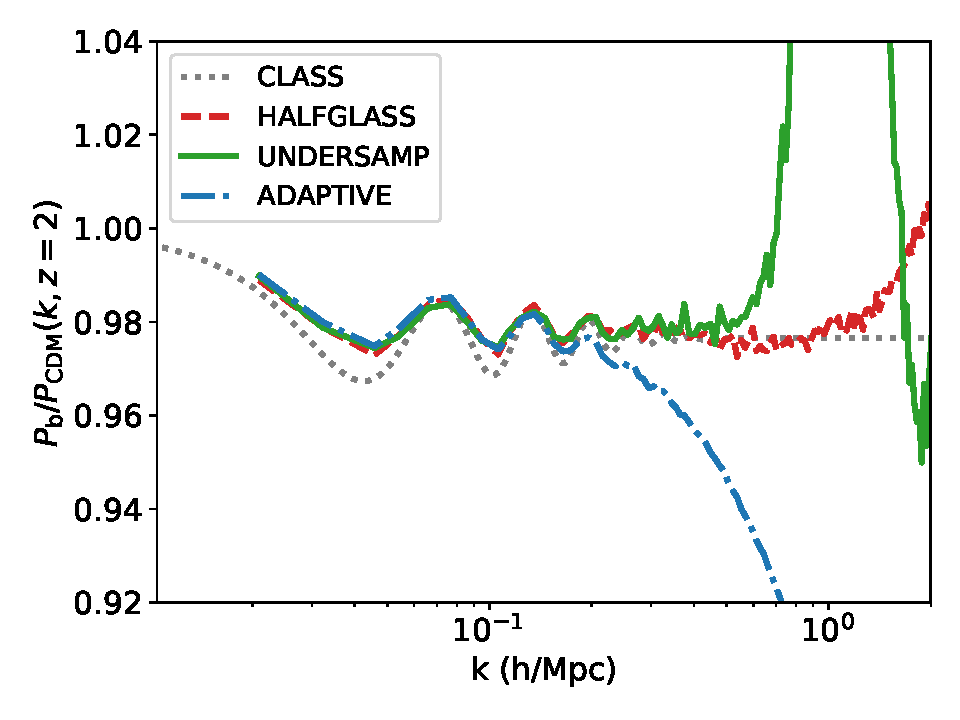
\includegraphics[width=0.5\textwidth]{plots/oversample_2_relpower.pdf}
  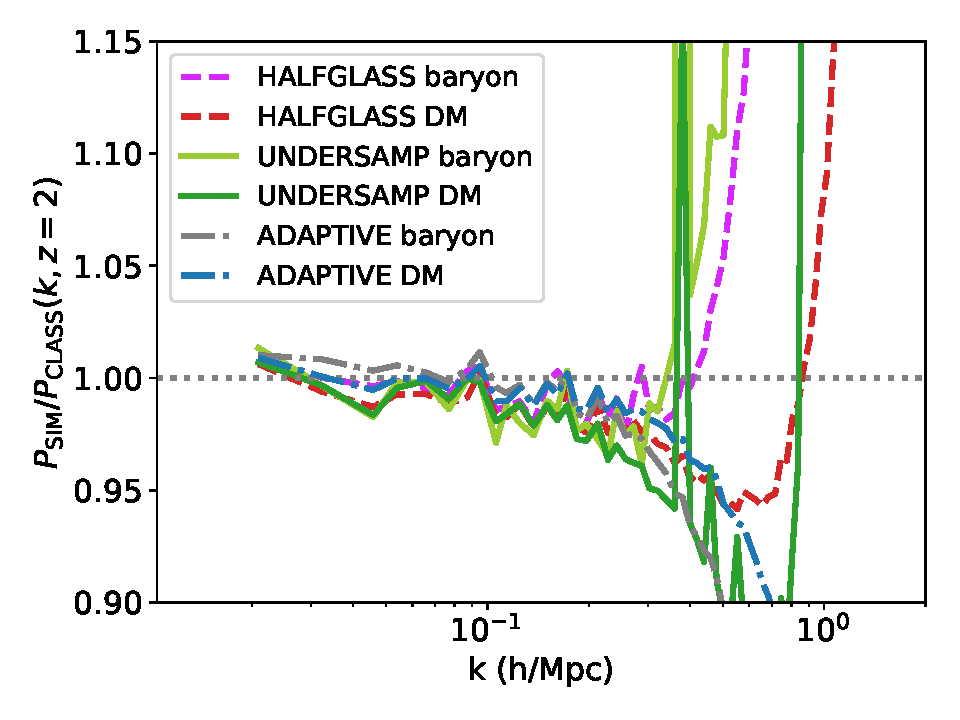
\includegraphics[width=0.5\textwidth]{plots/oversample_2_class.pdf}
\caption{Results for other simulation strategies successful at reproducing the relative power of baryons and CDM. Shown are: (ADAPTIVE) initializing particles on two regular grids, offset by half a grid spacing, but with particles evolved using an adaptive softening length for the gas. (UNDERSAMP) Using two regular grids with the number of CDM particle $5$ times larger than the number of baryon particles. Also show is the HALFGLASS simulation, for comparison. We have set $\sigma_8 = 0.008$ so that structure growth is linear even at late times. (Left) Ratio of gas to CDM power spectra, $P_\mathrm{bar}/P_\mathrm{CDM}(k)$, at $z=2$ for the simulation (solid) and linear theory from CAMB (dash). (Right) Ratio of simulated to linear power spectra, $P_\mathrm{sim}/P_\mathrm{CLASS}(k)$ for gas (orange) and CDM (blue).}
  \label{fig:adaptive}
\end{figure}

\begin{figure}
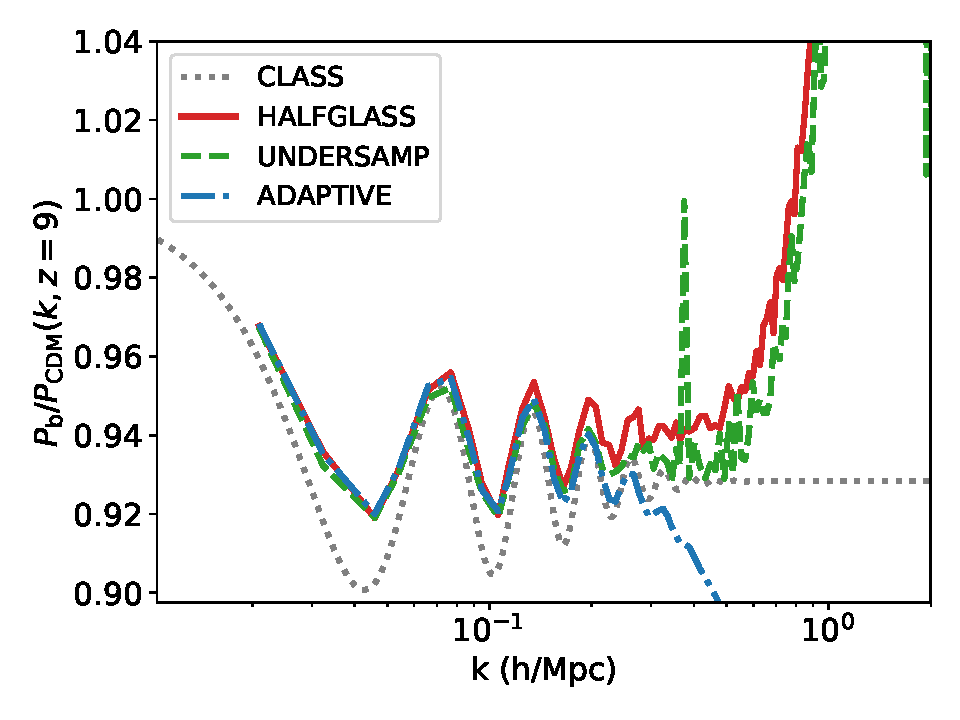
\includegraphics[width=0.5\textwidth]{plots/oversample_9_relpower.pdf}
  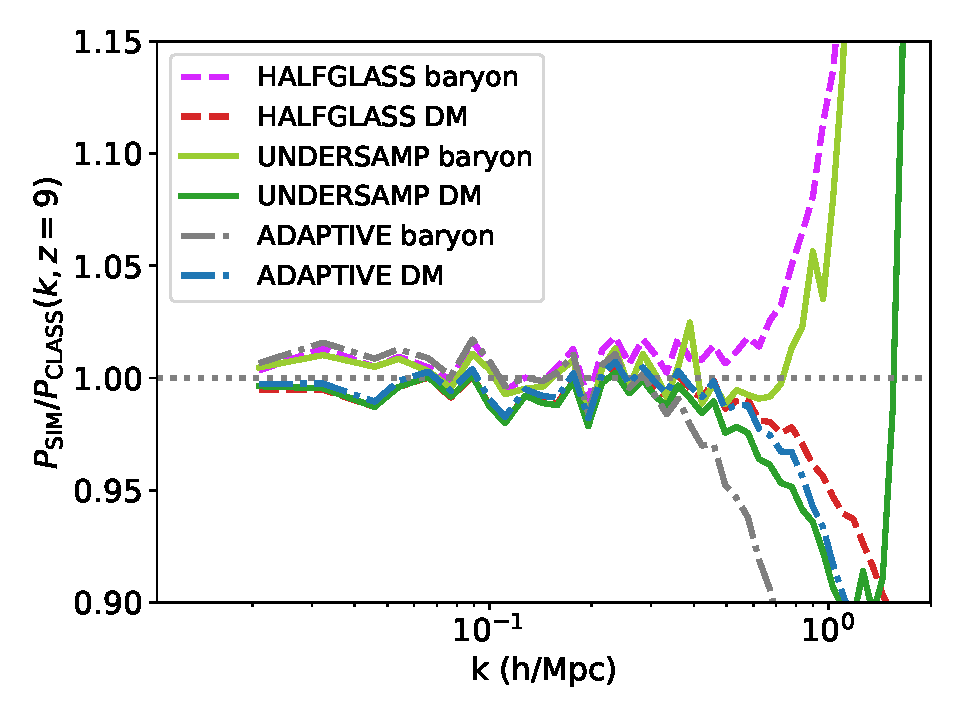
\includegraphics[width=0.5\textwidth]{plots/oversample_9_class.pdf}
\caption{Results for other simulation strategies successful at reproducing the relative power of baryons and CDM at $z=9$. Shown are: (ADAPTIVE) initializing particles on two regular grids, offset by half a grid spacing, but with particles evolved using an adaptive softening length for the gas. (UNDERSAMP) Using two regular grids with the number of CDM particle $5$ times larger than the number of baryon particles. Also show is the HALFGLASS simulation, for comparison. We have set $\sigma_8 = 0.008$. (Left) Ratio of gas to CDM power spectra, $P_\mathrm{bar}/P_\mathrm{CDM}(k)$, at $z=2$ for the simulation (solid) and linear theory from CAMB (dash). (Right) Ratio of simulated to linear power spectra, $P_\mathrm{sim}/P_\mathrm{CLASS}(k)$ for gas (orange) and CDM (blue).}
  \label{fig:adaptivez9}
\end{figure}


Figure~\ref{fig:offsetgrids} shows the baryon and cold dark matter power spectra for a cosmological simulation, compared to the output of CLASS at the same redshift. This simulation, TWOGRID, was initialized using the standard method of two grids of particles, one for baryons and one for cold dark matter, offset by a constant factor. Figure~\ref{fig:offsetgrids} illustrates the problem we aim to solve. Although the total matter power spectrum obeys the linear predictions, scattering between the baryon and DM particles causes the DM power spectrum to be over-predicted and the baryon power spectrum to be under-predicted, leading to an error in the relative power spectrum.
\AFR{Do we really understand why the measured high-k power is below linear theory? I find it very suspicious.}\spb{It is not really suspicious: it is just the 1-halo term from the particle grid. I will mark the Nyquist frequency on the plot and then it will be clearer.}
This problem has been discussed in, for example, Ref.~\cite{Angulo:2013}, although the magnitude of the error in our simulation does not match their results, presumably because of differences in the setting up of the regular grid.\footnote{\cite{Angulo:2013} have more power in the baryon component than linear theory predicts. For a similar simulation, we find less power than predicted by linear theory. It is unclear why this discrepancy occurs, but it seems likely to be due to differences in the initial velocity distribution or the exact setup of the initial particle grid.}

We have confirmed that these results are independent of the force accuracy of the simulation and are not connected to adaptive timestepping or the length of the timesteps. For the former, we have performed small simulations where the short range force was evaluated using an $N^2$ pairwise gravity solver, simulations where the tree opening angle was changed and simulations where the split scale between the short and long-range forces was altered. Although the total power in the box in some cases changed (to the extent expected given the new force accuracy) on small scales, the power ratio between the baryons and cold dark matter did not.
We also confirmed that our results were the same when all particles had the same timestep and when the long-range PM timestep was $4$ times shorter. We have also confirmed that our results are independent of box size and particle number.

Figure~\ref{fig:baryonglass} shows the baryon and cold dark matter power spectra for cosmological simulations initialized using a glass for the baryons, generated using the procedure described in Section~\ref{sec:glass}. The agreement with linear theory is substantially improved, demonstrating that a Lagrangian glass can suppress the unphysical scattering between the baryonic and DM particles.

This result may at first appear puzzling. Effects of the particle grid should be confined to small scales close to the mean inter-particle separation. However, because the grid structure is repeated across the whole box, each baryonic particle encounters the same scattering force, and so the effect is also replicated across the box and shows up as a scale-independent error. \YF{Alternatively speaking, there is a non-linear growth term that is proportional to the phase-angle between baryon and CDM. If they started from coherent grids, that cross term is larger than the realistic case, and produces a bias at all scales. $d_{bNL} = d_{b} + ... + (\alpha d_b + \beta d_cdm) <d_{b}, d_{cdm}> + ...$ $\alpha, \beta$ does depend on the type of gravity solver and mass difference.}

Using a Lagrangian glass for the baryons does not completely prevent unphysical force scatterings, but, because the particles are distributed irregularly, it ensures that the effect of this scattering is confined to small scales and does not change the large-scale growth. The glass does produce a noise power proportional to $k^4$ which in our case causes spurious small-scale growth. Since these are caused by the baryons, they would however be suppressed in a realistic simulation following gas pressures. We have performed a simulation with $\sigma_8 = 0.8$ with very similar results as Figure~\ref{fig:baryonglass}, demonstrating that our results are not being affected by the relatively large glass noise.
\AFR{How about running a simulation with hydro on? I'm really worried about how bad the power is at k=0.5 h/Mpc. We argue that the noise would be lower with hydro, but I'm not sure how much to trust this without running an actual test.}

As described in appendix B of Ref.~\cite{OLeary:2012}, the unphysical scatterings shown in Figure~\ref{fig:offsetgrids} occur because of the unequal particles masses, which allow dark matter particles to occasionally capture individual baryon particles. This motivates
an alternative solution to the relative power spectrum problem: changing the relative numbers of DM and baryon particles so that the per-particle mass is the same. For equivalent particle load this reduces the spatial resolution in the baryons by a factor of $\Omega_\mathrm{CDM}/\Omega_\mathrm{b} \sim 5$, which may not be desirable. However, it completely avoids the problem of unphysical particle captures and scatterings and, unlike the Lagrangian glass, does not introduce $k^4$ noise. Figure~\ref{fig:adaptive} shows the results of a simulation using this technique, confirming that it is also able to reproduce the baryon to DM power spectrum ratio on large scales at the cost of some Poisson noise in the power spectrum arising from poorer sampling.

Figure~\ref{fig:adaptivez9} shows the results of our simulations at $z=9$, where the linear theory transfer functions differ substantially more. Agreement is noticeably worse at $z=9$, especially for the baryons. This is expected: at $z=9$ the total clustering from structure is a factor of $0.09$ smaller than at $z=2$, and thus the  glass noise dominates at larger scales. The agreement is still reasonable \spb{Can I subtract the glass noise?} for the glass noise simulation. The simulation in which baryons are undersampled suffers from substantial sampling noise due to the large number of Fourier modes which do not contain any particles. All simulations agree for the cold dark matter.

Finally, we have checked that simulations which include adaptive gravitational softenings or disable the short-range tree force both reproduce the linear theory power spectra ratios on large scales, as suggested by Ref.~\cite{Angulo:2013}. Adaptive gravitational softenings avoid unphysical scatterings because the gravitational force is suppressed on scales less than that of the long-range particle mesh grid (in our simulations, 1/2 the mean interparticle spacing). Note that at high redshift, when the particle distribution is homogeneous, adaptive gravitational softenings are equivalent to disabling the short-range tree force.
Figure~\ref{fig:adaptive} shows the results, demonstrating that the loss of resolution is similar to undersampling the baryonic particles. Note that if a single particle is of sufficiently low mass to be Jeans stable, adaptive softenings are the physical thing to do \cite{Fire2:2018}. However, our simulations are of relatively low resolution and our particles are not near this threshold.

Compared to our preferred technique of using a Lagrangian glass for the baryonic particles, Figure~\ref{fig:adaptive} shows that both baryon undersampling and adaptive softenings produce similar results for the power spectrum. We prefer the use of Lagrangian glass because undersampling of baryons will negatively affect star formation models (which would be under-resolved), while using adaptive softenings leads to poor resolution in low-density areas, such as those which give rise to the \Lya~forest.

\subsection{Lyman-Alpha Forest Flux Power Spectrum}
\label{sec:lymanalpha}

% \begin{figure}
% 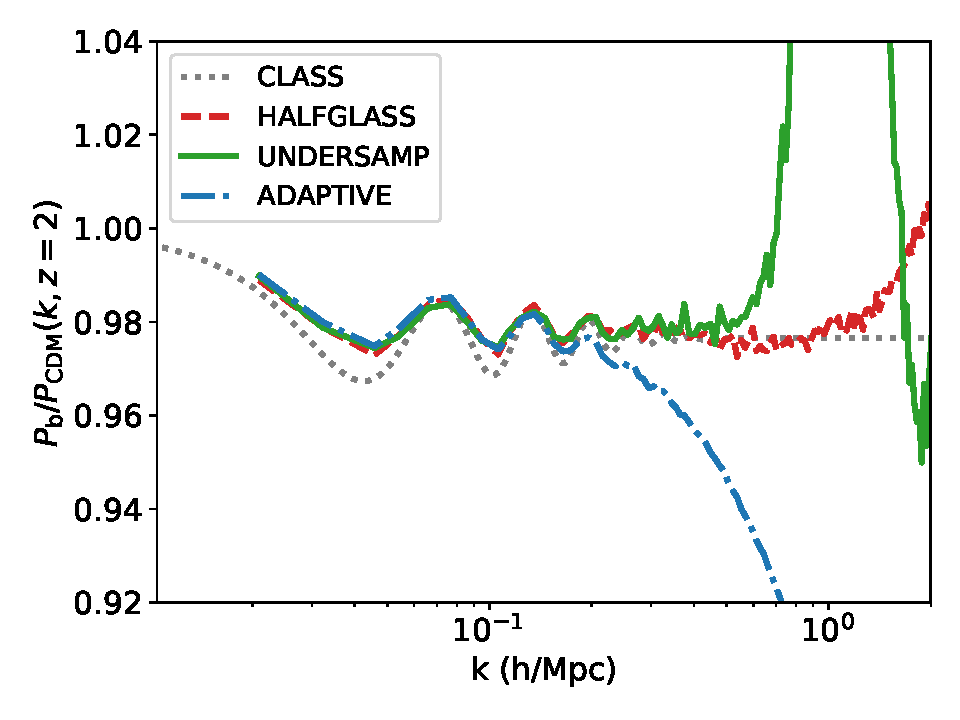
\includegraphics[width=0.5\textwidth]{plots/oversample_2_relpower.pdf}
%   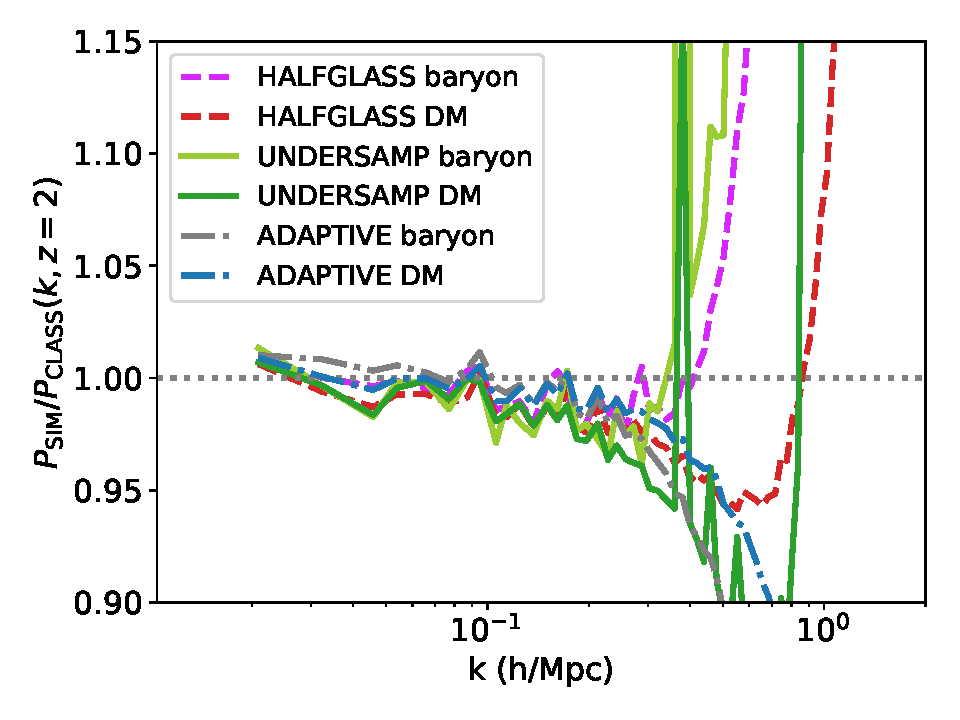
\includegraphics[width=0.5\textwidth]{plots/oversample_2_class.pdf}
% \caption{Results for a $120$ h/Mpc simulation with $512^3$ particles as used for the \Lya~forest. (Left) Ratio of gas to CDM power spectra, $P_\mathrm{bar}/P_\mathrm{CDM}(k)$, at $z=2$ for the simulation (solid) and linear theory from CAMB (dash). (Right) Ratio of simulated to linear power spectra, $P_\mathrm{sim}/P_\mathrm{CLASS}(k)$ for gas (orange) and CDM (blue).}
% \label{fig:lyamatter}
% \end{figure}

\begin{figure}
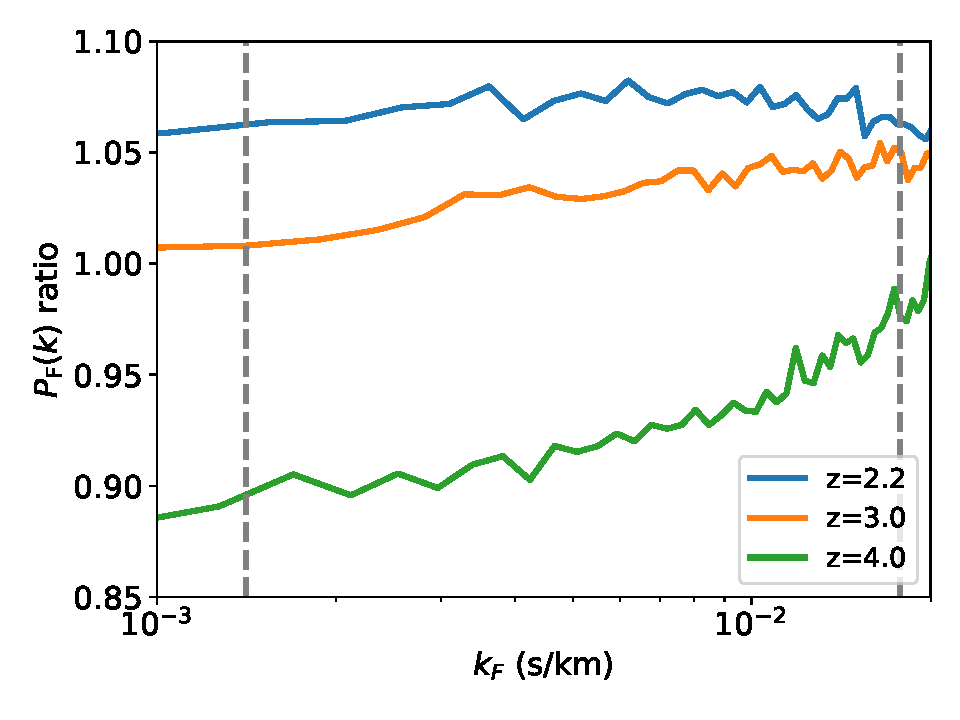
\includegraphics[width=0.5\textwidth]{plots/lya120_relflux_nomf.pdf}
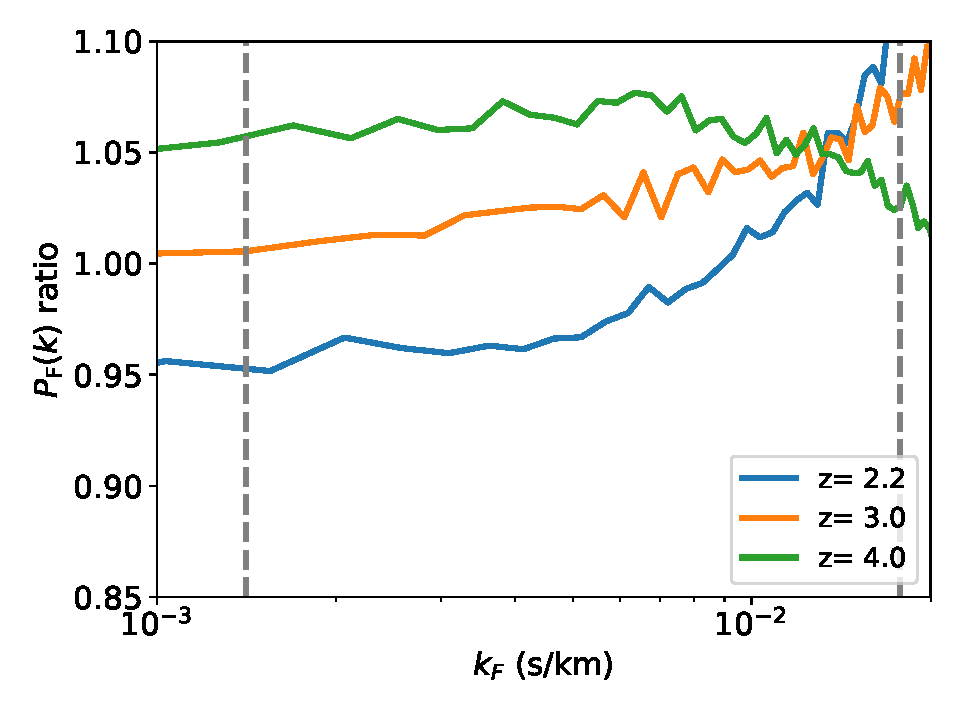
\includegraphics[width=0.5\textwidth]{plots/lya120_relflux_mf_t0.pdf}
\caption{Effect of separate transfer functions on the \Lya~forest flux power spectrum. Shown is $P_F(\mathrm{species})/P_F(\mathrm{total})(k)$, so that the reduction in baryon power due to a species-dependent transfer function produces $P_F(k) \mathrm{ratio} < 1$. (Left) The raw change in the flux power between the two simulations. (Right) The change in the flux power after scaling so that each simulation has the same temperature and mean flux. Vertical lines show the scales measured by SDSS/BOSS.
}
\label{fig:lyaflux}
\end{figure}

Thus far we have used idealised simulations in which the baryons are purely gravitational: pressure forces have been disabled. In this section we show how much separate transfer functions affect a realistic multiple fluid simulation of the \Lya~forest. We have performed two simulations with $\sigma_8 = 0.8$, $2\times 512^3$ particles and a $60$ h/Mpc box, standard parameters for resolving the \Lya~forest flux power spectrum. One simulation (FOREST) uses different transfer functions for the baryons and CDM, a grid for the CDM and a glass for the baryons. The other (TOTFOREST) uses the total matter power spectrum for both species \spb{Should I use a halfglass for that too? I think yes.}.
We checked explicitly that these
%Figure~\ref{fig:lyamatter} shows the relative matter power spectra (compared to linear theory) for the box with separate transfer functions, and demonstrates that we still achieve reasonable results for a full hydro simulation.

Figure~\ref{fig:lyaflux} shows the relative one dimensional \Lya~forest flux power spectrum for the simulation with separate transfer functions compared to the simulation without, and shows the total overall impact of neglecting the difference between particle species on a modern probe of structure formation. We also show the effect with the spectra scaled to produce the same \Lya~forest mean flux, as is standard practice when performing \Lya~forest analyses to marginalise uncertainty in the number density of intergalactic ionizing photons.

\section{Conclusions}
\label{sec:conclude}

We have shown that the spurious coupling present in N-body simulations between unequal mass CDM and baryon particles can be prevented from affecting the large scale power by setting the initial distribution of baryon particles with a Lagrangian glass. The CDM is initially placed on a grid. Chance juxtapositions of CDM and baryons are avoided by evolving the combined particle distribution with a reversed gravitational force, as in glass generation. This procedure allows a simulation to reproduce linear expectations for the power spectrum ratio between different particle species while avoiding the suppression of small scale power that results from increasing the gravitational softening length. We also explain an alternative possibility: over-sampling the CDM particles so that each particle species has the same mass, and demonstrate that this also reproduces linear expectations for the power spectrum ratio between different particle species.

\acknowledgments

We thank Tom Kitching, Yin Li, Pat McDonald, Matt McQuinn, Jose Onorbe, Andrew Pontzen, Martin Rey, Francisco Villaescusa-Navarro and Matias Zaldarriaga for helpful discussions. SB was supported by NSF grant AST-1817256. Computing resources were provided by NSF XSEDE allocation AST180058.

\bibliographystyle{JHEP}
\bibliography{offset}
\end{document}
